\documentclass{beamer}
\usetheme{Madrid}
\usepackage{booktabs}
\usepackage{tikz}
\usetikzlibrary{positioning}
\title{Early-Season Underdogs}
\subtitle{A public-data audit of Spencer's betting theory}
\author{Codex research brief}
\date{2026-04-09}

\begin{document}

\begin{frame}
\titlepage
\end{frame}

\begin{frame}{Question}
\begin{itemize}
\item Does betting every early-season underdog at closing moneyline odds make money?
\item Sample: NFL, NBA, NHL, MLB from 2011 through 2021.
\item Standard: transparent, public, reproducible, uncertainty-aware.
\end{itemize}
\end{frame}

\begin{frame}{Why This Could Work}
\begin{itemize}
\item Preseason priors can be stale.
\item Sportsbooks and bettors may update slowly after only a few games.
\item Small probability mistakes matter more for underdogs because payouts are
asymmetric.
\end{itemize}
\end{frame}

\begin{frame}{Data and Design}
\begin{itemize}
\item Public sportsbook archive snapshots from a documented GitHub repository.
\item 53,453 cleaned games across 44 league-seasons.
\item Main rules:
\begin{itemize}
\item first 2 weeks
\item first 3 weeks
\item first 5 games
\item first 10 percent of the team-season proxy
\end{itemize}
\item Primary stake: \$100 flat bet on every qualifying underdog.
\end{itemize}
\end{frame}

\begin{frame}{What Would Count as Evidence}
\begin{itemize}
\item Positive ROI after vig matters, but it is not enough on its own.
\item Beating all-season underdogs is suggestive.
\item The sharper test is calibration:
\begin{itemize}
\item did underdogs win more often than the no-vig market implied?
\end{itemize}
\item A confidence interval spanning losses and gains means the strategy is not
established as a reliable edge.
\end{itemize}
\end{frame}

\begin{frame}{Pipeline Diagram}
\centering
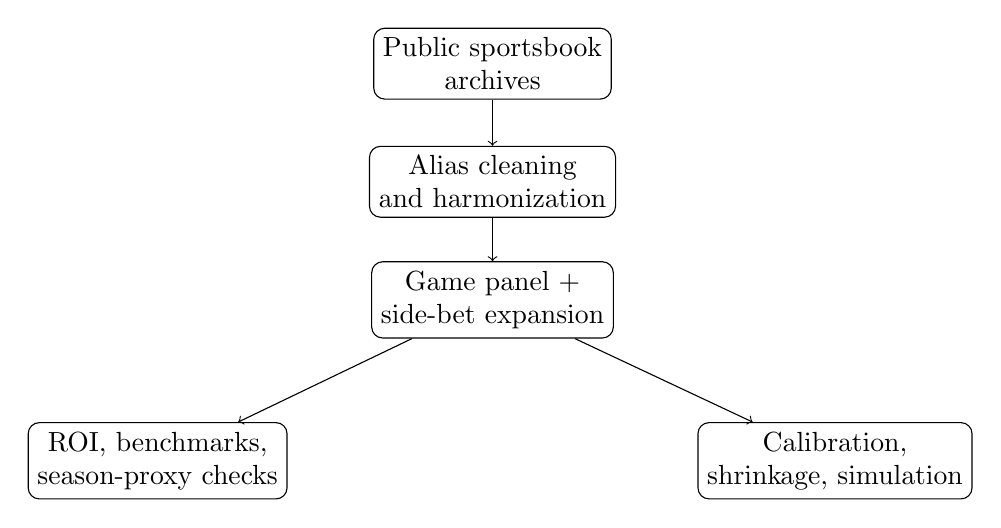
\begin{tikzpicture}[node distance=1.5cm, every node/.style={draw, rounded corners, align=center}]
\node (src) {Public sportsbook\\archives};
\node (clean) [below of=src] {Alias cleaning\\and harmonization};
\node (panel) [below of=clean] {Game panel +\\side-bet expansion};
\node (analysis) [below left=of panel] {ROI, benchmarks,\\season-proxy checks};
\node (model) [below right=of panel] {Calibration,\\shrinkage, simulation};
\draw[->] (src) -- (clean);
\draw[->] (clean) -- (panel);
\draw[->] (panel) -- (analysis);
\draw[->] (panel) -- (model);
\end{tikzpicture}
\end{frame}

\begin{frame}{Headline Results}
\begin{tabular}{lrr}
\toprule
Rule & ROI & Bets \\
\midrule
Underdogs, first 3 weeks & -0.4\% & 5,901 \\
All underdogs, likely-regular-season proxy & -1.8\% & 49,850 \\
Favorites, first 3 weeks & -4.1\% & 5,900 \\
\bottomrule
\end{tabular}

\vspace{0.4cm}

95\% bootstrap interval for the headline rule: [-4.0\%, 3.4\%].

\vspace{0.2cm}

Reading rule: the estimate is near breakeven, and the interval still includes
meaningful losses and modest gains.
\end{frame}

\begin{frame}{League Split}
\begin{tabular}{lrr}
\toprule
League & ROI & Read \\
\midrule
MLB & +3.9\% & positive hint \\
NFL & +1.8\% & noisy hint \\
NBA & -0.4\% & near zero \\
NHL & -8.2\% & negative \\
\bottomrule
\end{tabular}
\vspace{0.5cm}

These are noisy raw estimates. Partial pooling shrinks them back toward a
slightly negative pooled mean.
\end{frame}

\begin{frame}{Calibration Evidence}
\begin{itemize}
\item Early 3-week underdogs:
\begin{itemize}
\item realized win rate: 40.45\%
\item no-vig implied win probability: 39.70\%
\item calibration gap: +0.75 percentage points
\end{itemize}
\item Interpretation:
\begin{itemize}
\item some mild early underpricing may be present
\item the gap is too small to create a robust cross-league profit claim after vig
\end{itemize}
\end{itemize}
\end{frame}

\begin{frame}{Bottom Line}
\begin{itemize}
\item Early underdogs slightly outperform their own implied probabilities.
\item The effect is too small and unstable to claim a durable cross-league edge.
\item Best reading:
\begin{itemize}
\item weak support for mild early mispricing
\item strongest in MLB and maybe NFL
\item no credible all-league profit claim
\end{itemize}
\end{itemize}
\end{frame}

\end{document}
